\documentclass[10pt]{beamer}

\usepackage[utf8]{inputenc}
\usepackage[english,russian]{babel}

\usetheme[
  sectionpage=simple,
  numbering=fraction
]{metropolis}
\usepackage{appendixnumberbeamer}

\usepackage{numprint}
\usepackage{booktabs}
\usepackage[scale=2]{ccicons}

\usepackage{pgfplots}
\usepackage{listings}
% \usepackage{caption}
% \captionsetup[figure]{font=small}
\usepgfplotslibrary{dateplot}

\usepackage{xspace}
\newcommand{\themename}{\textbf{\textsc{metropolis}}\xspace}

\usepackage{todonotes}
\usepackage{ifthen}%
\providecommand\enabletodos{true}%
\ifthenelse{ \equal{\enabletodos}{true} }{%
  \presetkeys{todonotes}{inline}{}%
}{%
  \presetkeys{todonotes}{disable}{}%
}%

\setbeamertemplate{caption}{\raggedright\insertcaption\par}

\AtBeginSection[]{}

\setbeamertemplate{section in toc}{%
  \alert{$\bullet$}~\inserttocsection}
\setbeamercolor{subsection in toc}{bg=white,fg=structure}
\setbeamertemplate{subsection in toc}{%
  \hspace{1.2em}{\alert{\rule[0.3ex]{3pt}{3pt}}~\inserttocsubsection\par}}

\usepackage{hyperref}
\hypersetup{unicode=true}

\usepackage{tikz}
\usepackage{forest}
\usetikzlibrary{arrows,positioning}
\tikzset{
    % Define standard arrow tip
    >=latex,
    % Define arrow style
    ptr/.style={->, thick},
}
\usepackage{drawstack}
\usepackage{adjustbox}
\protected\def\psverb#1{\def\innerpsverb##1#1{\texttt{##1}}\innerpsverb}
\usepackage{listings}

\usepackage{makecell}

\usepackage[noline, noend]{algorithm2e} % For algorithms
\SetAlFnt{\footnotesize}

\usepackage{float}

\usepackage{changepage}
% \usepackage{pscyr} % Нормальные шрифты
 
% \usepackage{algorithm}
% \usepackage{algpseudocode}

\lstdefinestyle{C}{
  language=C,
  % numbers=left,
  stepnumber=1,
  % numbersep=10pt,
  % tabsize=4,
  showspaces=false,
  showstringspaces=false
}
\lstset{basicstyle=\tiny,style=C}


\metroset{block=transparent}
\definecolor{Blue}{HTML}{2375a8}
\setbeamercolor{frametitle}{bg=Blue}
\setbeamercolor{palette primary}{bg=Blue}


\definecolor{Blue2}{HTML}{9ccff0}
\setbeamercolor{block title}{bg=Blue2}

\title{Магистерская диссертация}
\subtitle{Исследование и разработка методов динамического анализа для определения входных данных влияющих на выполнение условных переходов}
\author{Дьячков Л.А.\\[3mm]{\small Руководитель: д.ф-м.н, профессор. Петренко А.К.}\\[1mm]
{\small Cоруководитель: к.ф-м.н, с.н.с. Курмангалеев Ш.Ф.}\\[3mm]
}
\institute{ИСП РАН}
\date{17 Июня 2019}
\titlegraphic{\hfill
\includegraphics[height=0.5cm]{logo_isp_ru.png}}

\begin{document}

\maketitle


% \begin{frame}{Введение}
%   \begin{block}{Фаззинг}
%   \textbf{Фаззинг-тестирование} -- активно развивающийся метод для поиска ошибок в программном обеспечении %\cite{DBLP:journals/corr/abs-1808-09700}.
%   \end{block}
%   \pause
%   \begin{block}{Проблема}
%   Может быть затруднено нахождение входных данных, позволяющих ``пройти'' условный переход
%   \end{block}
%   \pause
%   \begin{block}{Предлагаемое решение}
%     Использовать методы динамического анализа для определения какие байты из входного файла влияют на конкретный условный переход
%   \end{block}
% \end{frame}

\begin{frame}{Введение}
  \begin{block}{Фаззинг}
  \textbf{Фаззинг-тестирование} -- активно развивающийся метод поиска ошибок в программном обеспечении, основанный на автоматической генерации входных данных с целью поиска аварийных завершений.
  \end{block}

  \begin{block}{Актуальность}
  Слабым местом фаззинг-тестирования является подбор входных данных для прохождения сложных условных переходов. Необходимы методы, которые позволят фаззеру эффективнее справляться с данной задачей.

  \end{block}
\end{frame}

\begin{frame}{Постановка задачи}

Цели работы
\begin{itemize}
    \item Исследовать методы динамического анализа с целью выявления подходов, применимых к задаче определения входных данных, влияющих на выполнение условных переходов.
    \item Провести анализ существующих инструментов динамического анализа с точки зрения применимости к решаемой задаче.
    \item Разработать методы определения входных данных, влияющих на выполнение условных переходов, на основе динамического символьного выполнения и на основе динамического анализа помеченных данных.
    \item Привести программную реализацию разработанных методов, провести её тестирование на наборе \texttt{LAVA} и программах с открытым исходным кодом.
\end{itemize}

  % \begin{block}{Цель работы}
  %   \begin{itemize}
  %   \item Разработка метода динамического анализа, позволяющего определять байты входного файла, влияющего на выполнение инструкции условного перехода.
  %   \item Программная реализация метода, работающая на операционной системе Linux с архитектурой процессора x86-64
  %   \end{itemize}
  % \end{block}
  % \pause

  % \begin{block}{Подзадачи}
  %   \begin{itemize}
  %     \item Изучение существующих технологий динамического символьного выполнение и динамического анализа потока данных.
  %     \item Сравнение технологий на тестовом наборе
  %     \item Обзор возможных подходов, реализация прототипов, разработка метода
  %     \item Программная реализация на основе выбранной технологии
  %   \end{itemize}
  % \end{block}

    % \textbf{Задача} Для сравнения инструментов использовать существующию инфраструктуру Google OSS-fuzz \\
    % \textbf{Результаты}
    % \begin{itemize}
    %   \item Изучена инфраструктура google os fuzz.
    %   \item Получено представление о работе afl и libfuzz (в меньшей степени) c точки зрения пользователя
    %   \item На jenkins заведен job, запускающий afl фаззер при помощи oss fuzz
    %   \item Понимание как адаптировать имеющуюся инфраструктуру для оценки инструментов taint анализа не получено
    % \end{itemize}
\end{frame}
%}%

\begin{frame}{Динамическое символьное выполнение}
  \begin{block}{Определение}
    Метод динамического анализа, заключающийся в том, что во время выполнения программы некоторым конкретным значениям ставятся в соответствие символьные переменные. Затем для каждой выполняемой инструкции генерируются формулы для SMT-решателя.
  \end{block}
  \begin{block}{Online символьное выполнение}
    Модуль символьного выполнения используется для того, чтобы генерировать конкретные данные для посещения новых узлов ГПУ программы.
  \end{block}
  \begin{block}{Offline символьное выполнение}
    Модуль символьного выполнения используется для анализа конкретной трассы выполнения. \checkmark
  \end{block}
\end{frame}


\begin{frame}{Динамический анализ помеченных данных}
  \begin{block}{Определение}
    Динамический анализ помеченных данных (Dynamic Taint Analysis), также известный как динамический анализ потока данных (Dynamic Flow tracking) -- это техника анализа програм, позволяющая определить какие состояния программы зависят от входных данных.
  \end{block}
  \begin{block}{Принцип работы}
    \begin{itemize}
        \item {\em Определение источников помеченных данных}. Обычно метками снабжаются данные, получаемые из недоверенного источника (файл, stdin, сеть).
        \item {\em Распространение пометок (Taint propagation)}. Для каждой инструкции необходимо принять решение, как распространяются пометки в зависимости от её операндов и факта их помеченности.
        % \begin{itemize}
        %     \item Следует ли отслеживать помеченность побайтово или побитого? Если \textint{eax} помечен, то после команды \textint{or eax, 0x746567bc} контролируются уже не все биты. Однако, в большинстве случаев отслеживание каждого бита может быть слишком дорогой операцией.
        %     \item Следует ли помечать адрес памяти, на который указывает помеченная переменная?
        %     \item Если условный переход зависит от помеченных данных, следует ли считать что последующие инструкции тоже от них зависят?
        %     \item Как хранить информацию о помеченных адресах в памяти?
        %     \item Cледует ли различать пометки, полученные из разных источников?
        % \end{itemize}
        \item {\em Применение политик безопасности}. Например, отслеживание попадания помеченных данных в аргументы ``опасных'' функций или факта помеченности счетчика инструкций.
    \end{itemize}
  \end{block}
\end{frame}

% \begin{frame}{Проблема распространения пометок}
%     \begin{itemize}
%         \item Следует ли отслеживать помеченность побайтово или побитого? Если \textit{eax} помечен, то после команды \textit{or eax, 0x746567bc} контролируются уже не все биты. 
%         \item Следует ли помечать адрес памяти, на который указывает помеченная переменная?
%         \item Если условный переход зависит от помеченных данных, следует ли считать что последующие инструкции тоже от них зависят?
%         \item Как хранить информацию о помеченных адресах в памяти?
%         \item Cледует ли различать пометки, полученные из разных источников?
%     \end{itemize}
% \end{frame}

\begin{frame}{Исследованные технологии}
  \begin{block}{Динамическое символьное выполнение}
    \begin{itemize}
      \item Triton
      \item Angr
      \item Manticore
    \end{itemize}
  \end{block}
    \begin{block}{Динамический анализ помеченных данных}
    \begin{itemize}
      \item Triton 
      \item Taintgrind
      \item libdft64
      \item Moflow gentrace
    \end{itemize}
  \end{block}
\end{frame}

\begin{frame}{Triton}
    Среда для динамического анализа исполняемого кода, поддерживает архитектуры x86 и x86-64, содержит модули DSE (offline) и анализа помеченных данных, использует \emph{Intel Pin} для динамической бинарной инструментации.
    \begin{block}{Достоинства}
        \begin{itemize}
        \item Поддерживает offline режим динамического символьного выполнения.
        \item Имеет режим, позволяющий генерировать SMT формулы только для помеченных инструкций.
        \end{itemize}
    \end{block}

      \begin{block}{Недостатки}
          \begin{itemize}
      \item На два порядка медленее других инструментов на базе Pin
      \item Нет поддержки символьных файлов/помечивания данных на основе системных вызовов.
      \item Отслеживает только сам факт помеченности данных, нет возможности различать источники.
      \end{itemize}
    \end{block}

\end{frame}

% \begin{frame}{Triton | Достоинства}
%     \begin{itemize}
%         \item Поддерживает offline режим динамического символьного выполнения (Нет необходимости предварительно снимать трасу, при помощи pin это делается ``на лету'')
%         \item Поддерживает \textbf{"ONLY\_TAINTED"}, позволяющий генерировать smt формулы только для
%         \item Богатое и документированное api c множеством примеров.
%         \item Поддерживает интерфейс для использования средств динамической бинарной инструментации, отличных от pin
%     \end{itemize}
% \end{frame}

% \begin{frame}[fragile]{Triton | Недостатки}
%       \begin{itemize}
%       \item 
%       \item Генерирует громоздкие SMT формулы для SSE инструкций. Предикат пути для примера ниже не решается в течение месяца.
%       \begin{verbatim}
%         for (int i = 0; i < arg_length; i++) {
%             buff[i] = (++argv[1][i]);
%         }
%         if (!strncmp(buff, "/home/", 6))
%         \end{verbatim}
%       \item Нет поддержки символьных файлов/пометки данных на основе системных вызовов.
%       \item Cодержит ошибки в реализации обработчиков нескольких инструкций
%       \begin{itemize}
%               \item Ошибка распространения пометов для инструкции \textbf{pcmpeqb} https://github.com/JonathanSalwan/Triton/issues/730
%               \item Неверный предикат пути для инструкции \textbf{repe cmpsb}
%           \end{itemize}
%       \end{itemize}
% \end{frame}

\begin{frame}{Angr}
    Платформонезависимая среда динамического символьного выполнения, использующая трансляцию инструкций в VEX с последующей эмуляцией.
    \begin{block}{Достоинства}
      \begin{itemize}
        \item Поддержка множества архитектур.
        \item Многофункциональный модуль online символьного выполнения, отлично работающий поиск состояний на небольших примерах.
        \item Есть множество полезных примитивов (таких как символьные файлы) из коробки.
      \end{itemize}
    \end{block}
        \begin{block}{Недостатки}
          \begin{itemize}
      \item Нет offline-режима (плагины, которые должны его поддерживать не работают).
      \item На настоящих (например GNU binutils) программах online-поиск не может дойти до интересных состояний.
      \end{itemize}
    \end{block}
\end{frame}


\begin{frame}{Manticore}
    Аналог Angr, поддерживающий также анализ смарт-контрактов для Ethereum. Использует эмуляцию инструкций.
    \begin{block}{Достоинства}
      \begin{itemize}
        \item Поддерживает offline-режим. % на самом деле нет
      \end{itemize}
    \end{block}
        \begin{block}{Недостатки}
          \begin{itemize}
      \item Низкая производительность (требуется 50 секунд эмуляции для того, чтобы дойти до main в программе с glibc).
      \item Нет поддержки SSE инструкций.
      \item Нет поддержки некоторых системных вызовов при эмуляции.
      \end{itemize}
    \end{block}
\end{frame}

\begin{frame}{Taintgrind}
    Плагин для valgrind, реализующий динамической анализ потока данных.
    \begin{block}{Достоинства}
      \begin{itemize}
        \item Поддержка множества архитектур (все, что поддерживает valgrind).
        \item Возможность помечать данные из конкретных файлов.
        \item Возможность статической инструментации исходного кода для пометки данных.
      \end{itemize}
    \end{block}
        \begin{block}{Недостатки}
          \begin{itemize}
      \item Отслеживает только сам факт помеченности данных, нет возможности различать источники.
      \end{itemize}
    \end{block}
\end{frame}

\begin{frame}{libdft64}
    Инструмент для динамического анализа помеченных данных, работающий на основе \emph{Intel Pin}. Реализация libdft (поддерживает только x86) из проекта vuzzer64 работающая с 64-разрядными исполняемыми файлами. 
    \begin{block}{Достоинства}
      \begin{itemize}
        \item Возможность помечать данные из конкретных файлов.
        \item Гранулярность меток на уровне байта.
      \end{itemize}
    \end{block}
        \begin{block}{Недостатки}
          \begin{itemize}
      \item Игнорируется регистр флагов.
      \item Поддерживаются не все инструкции.
      \end{itemize}
    \end{block}
\end{frame}


\begin{frame}{moflow gentrace}
    Инструмент для динамического анализа помеченных данных, работающий на основе \emph{Intel Pin}.
    Часть фреймворка moflow, изначально являющийся частью bap.
    \begin{block}{Достоинства}
      \begin{itemize}
        \item Возможность помечать данные из конкретных файлов.
        \item Гранулярность меток на уровне байта.
      \end{itemize}
    \end{block}
        \begin{block}{Недостатки}
          \begin{itemize}
      \item Отсутствие учета семантики инструкций в механизме распространения пометок.
      \item Использование специальной метки \emph{MIXED\_TAINT} в случае, если адрес зависит от нескольких пометок.
      \item Механизм распространения пометок работает на уровне старших регистров.
      \end{itemize}
    \end{block}
\end{frame}

\begin{frame}{Выбранные инструменты}
    \begin{block}{Динамическое символьное выполнение}
      Angr
    \end{block}
    \begin{block}{Динамический анализ помеченных данных}
        Moflow gentrace
    \end{block}
\end{frame}


\begin{frame}{Метод на основе символьного выполнения}

Каждому байту входного файла ставится в соответствие символьная переменная.
При добавлении на очередном условном переходе в предикат пути новой формулы, для неё выполняется следующий алгоритм:

\begin{algorithm}[H]
\SetAlgoLined
\KwIn{Предикат пути, представленный в виде AST для SMT формулы}
\KwOut{Список символьных переменных}
\SetKwFunction{getleafs}{\textbf{GetLeafs}}
\SetKwFunction{issymvar}{\textbf{IsSymVar}}
\SetKwFunction{isconstant}{\textbf{IsConstant}}
\SetKw{continue}{\textbf{continue}}
% \Indm\nonl\printlcs{$V$}\\
% \KwResult{Write here the result
\SetKwProg{Fn}{Function}{:}{}
\Fn{\getleafs{$V$}}{
$Found \gets \emptyset$\;
  \For{$child \in V$} {
    \If{$\issymvar ( child ) $} {
        $Found \gets Found \cup \{ child \}$\;
    } \ElseIf{$\isconstant ( child ) $} {
        $\continue$\;
    }
    \Else {
      $Found \gets Found \cup \getleafs{child}$\;
    }
  }
  \Return{$Found$}\;
}
  \caption{Метод на основе символьного выполнения}
\end{algorithm}
Поскольку переменные взаимнооднозначно соответствуют адресам -- задача решена.
\end{frame}

% \begin{frame}{Метод на основе символьного выполнения}

%   \begin{block}{Достоинства}
%     \begin{itemize}
%       \item Простой в реализации алгоритм
%       \item Высокая точность работы
%     \end{itemize}
%   \end{block}
%   \pause
%   \begin{block}{Недостатки}
%     \begin{itemize}
%       \item Низкая производительность (Построение формул на каждую инструкцию)
%       \item Ни один из расмотренных DSE инструментов не позволяет реализовать метод, работающий на несинтетических примерах без ощутимых доработок самого инструмента
%     \end{itemize}
%   \end{block}

% \end{frame}

\begin{frame}[fragile]{Реaлизация и тестирование}
Метод на основе динамического символьного выполнения был реализован на фреймворке \textbf{Angr}.

Программа успешно работает на следующем примере:
\begin{lstlisting}[basicstyle=\ttfamily\tiny]
int main(int argc, char** argv)
{
    char buff[SIZE];
    FILE *file1, *file2;
    file1 = fopen("input1", "r");
    file2 = fopen("input2", "r");
    fseek(file1, 10, SEEK_SET);
    fread(buff, sizeof(char), 7, file1)
    fread(buff, sizeof(char), 2, file2)
    if (buff[0] == 'a') {
        if (buff[3] == 'b') {
            loc1();
        } else if (buff[5] < buff[6]) {
            loc2();
        } else if (buff[2] >= buff[1]) {
            loc3();
        }
        loc4();
    }
    loc5();
    puts(buff);
}
\end{lstlisting}
Но не работает на более сложных (например программа cmark для генерации html из markdown).

\end{frame}

% \begin{frame}{Метод на основе символьного выполнения}

%   \begin{block}{Достоинства}
%     \begin{itemize}
%       \item Простой в реализации алгоритм
%       \item Высокая точность работы
%     \end{itemize}
%   \end{block}
%   \pause
%   \begin{block}{Недостатки}
%     \begin{itemize}
%       \item Низкая производительность (Построение формул на каждую инструкцию)
%       \item Ни один из расмотренных DSE инструментов не позволяет реализовать метод, работающий на несинтетических примерах без ощутимых доработок самого инструмента
%     \end{itemize}
%   \end{block}

% \end{frame}


\begin{frame}{Метод на основе анализа помеченных данных}

    \begin{itemize}
      \item Каждому байту входного файла ставится в соответствие метка (тег).
      \item Для всех инструкций в трассе выполняется алгоритм распространения меток.
      \item Для каждой инструкции условного перехода извлекаются теги, которыми помечен регистр флагов. Байты, соответствующие этим тегам -- искомые.
    \end{itemize}
\end{frame}

\begin{frame}[fragile]{Метод на основе анализа помеченных данных}

    \scalebox{0.35}{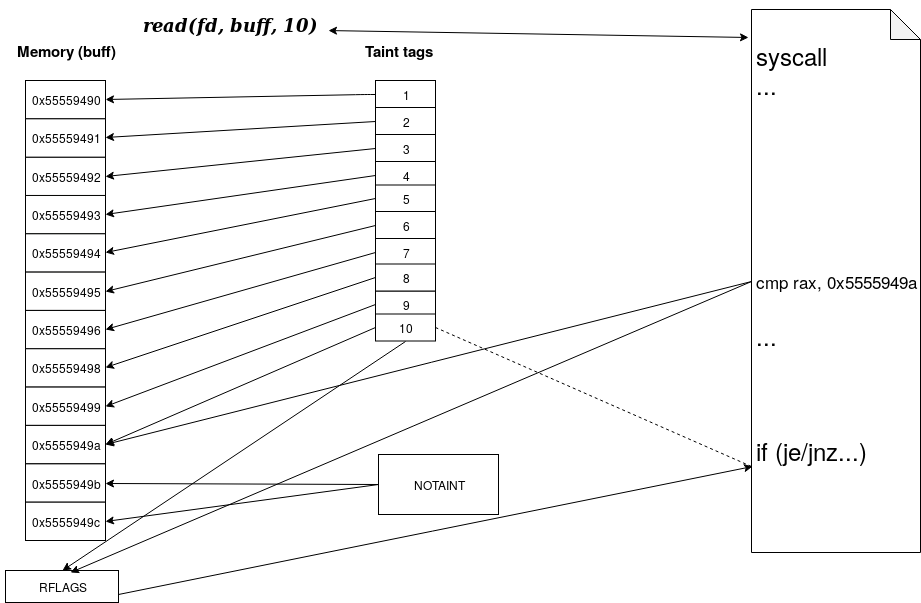
\includegraphics{../img/source_tainting.png}}

\end{frame}

% \begin{frame}{Метод на основе анализа помеченных данных}

% \begin{block}{Достоинства}
%   \begin{itemize}
%     \item Высокая скорость работы
%     \item Простая реализация
%   \end{itemize}
% \end{block}
% \pause
%   \begin{block}{Недостатки}
%     \begin{itemize}
%       \item Точность ниже чем у символьного выполнения.
%     \end{itemize}
%   \end{block}
% \end{frame}

\begin{frame}{Реaлизация}

Для реализации метода на основе анализа помеченных данных был выбран \texttt{Moflow gentrace}.

\end{frame}


\begin{frame}[fragile]{Доработки Moflow}
    % \hfill
    % {\scriptsize\input{mydrawio.pdf_tex}}
    \textbf{RCX} помечен $8$ тегами. Moflow бы пометил бы
    \textbf{RCX} как \textbf{MIXED\_TAINT}, для реализации множественного помечивания нужна структура \textbf{Множество пометок}.

    \scalebox{0.3}{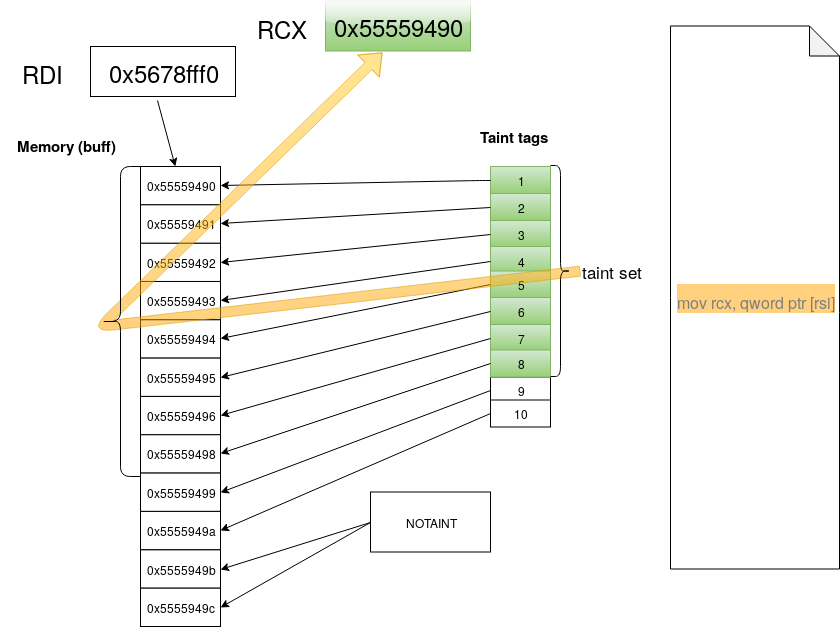
\includegraphics{../img/propagation1.png}}

\end{frame}

\begin{frame}[fragile]{Доработки Moflow}
    \textbf{0x5678fff0} и \textbf{0x5678fff1} помечаются $8$ тэгами. Правильно было бы представить \textbf{RCX} как 8 отдельных байт, которые могут быть помечены независимо, тогда \textbf{0x5678fff0} и \textbf{0x5678fff1} будут помечены $2$ различными тегами.
    \scalebox{0.25}{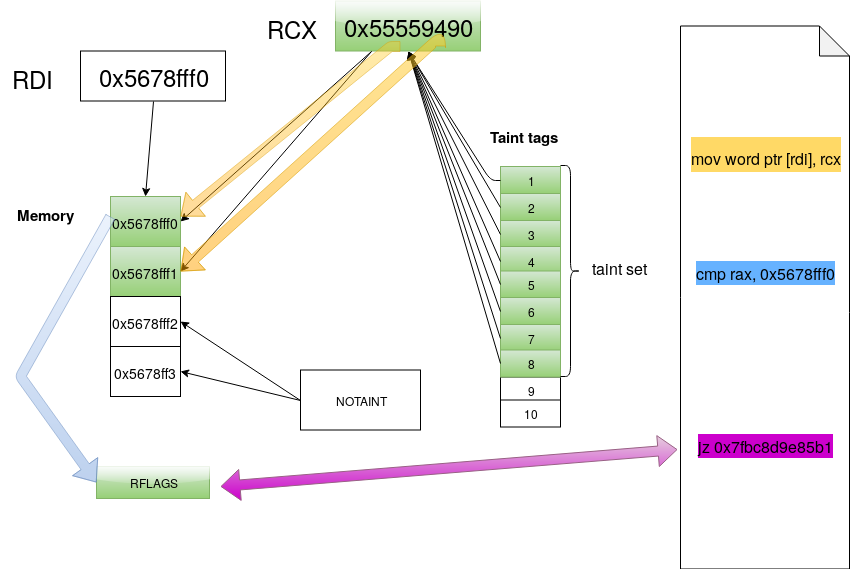
\includegraphics{../img/propagation2.png}}

\end{frame}


\begin{frame}{Доработки Moflow | Множество меток}
    
    \textbf{Множество меток} -- структура для поддержки множественных пометок, от неё требуется поддержка следующих операций:
    \begin{itemize}
        \item Добавление метки в \textbf{Множество меток}.
        \item Объединение с другим \textbf{Множеством меток}.
        \item Вывод содержимого \textbf{Множества меток}.
     \end{itemize}
     % \pause
     % Было разработано несколько подходов к реализации структуры.

\end{frame}

\begin{frame}{Доработки Moflow | Множество меток | Различные реализации }
    \begin{itemize}

        \item Динамический массив (\texttt{std::vector}).
        \item Битовое множество (\texttt{std::bitset}).
        \item Cжатое битовое множество (\texttt{Croaring}).
        \item Ассоциативный массив из битовых множеств (\texttt{std::map} из стандартной библиотеки, ключами которого являются целые числа, а значениями -- битовые вектора размера $N$).
        \item Множество интервалов \texttt{boost::icl::interval\_set}.
     \end{itemize}
     \pause
       Поскольку не менее 70\% операций объединения проводится над пустыми множествами и множествами из $1$ элемента, во всех случаях множество меток было реализовано как пара из \textbf{uint32\_t} и указателя на более сложную структуру (который в этих 70\% оказывается нулевым).

\end{frame}

\begin{frame}{Доработки Moflow | Множество пометок | Тестовые примеры}
\begin{itemize}
    \item \texttt{cmark} -- программа для преобразования markdown в HTML, написанная на \texttt{C}, входной файл из $3379$ байт, количество инструкций в трассе \numprint{608398}, количество операций над множествами меток \numprint{205273}.
    \item \texttt{file} -- инструмент из набора GNU coreutils, определяющий тип файла, входной файл содержит строку \texttt{``1123235235346436\textbackslash n''}, количество инструкций в трассе \numprint{14343775}, количество операций над множествами меток \numprint{23494644}.
    \item \texttt{jpeg} -- программа из набора \texttt{LAVA}  для обработки jpeg файлов, входной файл из $5770$ байт, количество инструкций в трассе \numprint{9043561}, количество операций над множествами меток \numprint{55839222}.
    \item \texttt{libyaml} -- программа из набора \texttt{LAVA} для обработки yaml файлов, входной файл из $5242$ байт, количество инструкций в трассе \numprint{11580028}, количество операций над множествами меток \numprint{11157748}.
\end{itemize}
\end{frame}

\begin{frame}{Доработки Moflow | Множество пометок}

    \textbf{Время работы в секундах для различных реализаций}\\
    \scalebox{0.65}{
    \begin{tabular}[]{@{}lllllllll@{}}
    \toprule
    & vanilla & vector & bitset6000 & roaring & bitset64 tree & bitset256
    tree & bitset512 tree & interval set \tabularnewline
    \midrule
    % \endhead
    cmark & 3.5s & 4.6s & 3.7s & 4.2s & 3.8s & 3.7s & 3.7s & 3.7s \tabularnewline
    file & 20.8s & 47s & 60s & 70s & 45.5s & 46s & 47s & 46s \tabularnewline
    libjpeg & 14.5s & 1762s & 49s & 378s & 307s & 108s & 80s & 165s \tabularnewline
    libyaml & 16.5s & 22.5s & 25s & 26s & 23.5s & 23.5s & 23.5s & 24s \tabularnewline
    \bottomrule
\end{tabular}}
\end{frame}

% \begin{frame}{Доработки Moflow | Другие доработки | удаление ненужного функционала}

% Целью изначального инструмента было сохранение трасс выполнения в формате \texttt{protobuf}, однако с точки зрения решаемой задачи в этом нет никакого необходимости.
% \pause
% \begin{table}[H]
%     \centering
%     \caption{Время работы с сериализацией и без} \label{tab:compare2}
%     % \scalebox{0.4}{
%     \begin{tabular}[]{@{}lll@{}}
%     \toprule
%     & с сериализацией трассы & без сериализации трассы  \tabularnewline
%     \midrule
%     % \endhead
%     cmark & 3.7s & 3.4s \tabularnewline
%     file & 46s & 29s \tabularnewline
%     libjpeg & 108s & 99s \tabularnewline
%     libyaml & 23.5s & 22s \tabularnewline
%     \bottomrule
% \end{tabular}
% \end{table}
% \pause
% \begin{itemize}
% \item производительность возрасла
% \item возможность использовать версию \texttt{Pin 3.7} по причине отсутствия внешних зависимостей.
%   \end{itemize}

% \end{frame}

\begin{frame}{Доработки Moflow | Другие доработки | Задание гранулярности меток}
\textbf{afl-analyze} --- инструмент, позволяющий определять контрольные суммы и магические значения во входных файлах.
% \pause
\begin{figure}[H]
    \center{
        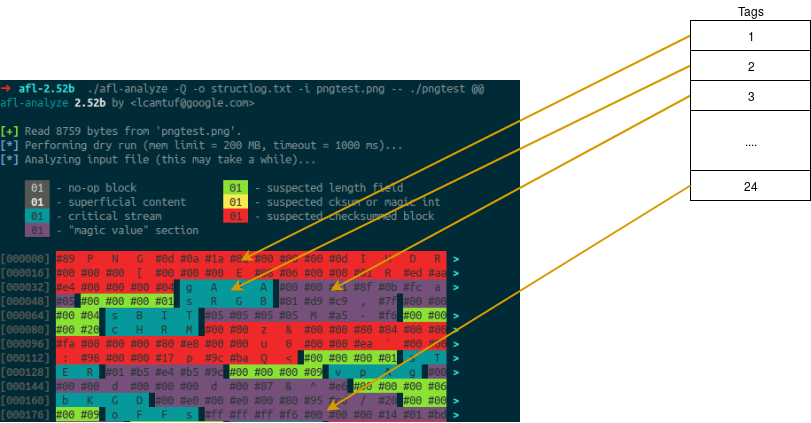
\includegraphics[scale=0.3]{../img/granularity.png}
    }
\end{figure}
Данные, для которых \texttt{afl-analyze} не смог определить семантику, помечаются обычным образом.
\end{frame}

\begin{frame}{Доработки Moflow | Итоги}
\begin{itemize}
 \item Добавлена поддержка множественного помечивания.
 \item Предложена эффективная структура данных для хранения множества меток.
 \item Добавлена возможность использования произвольной гранулярности меток, в том числе на основе afl-analyze.
 \item Добавлена поддержка новых системных вызовов для помечивания входных данных (\textbf{pread64}, \textbf{recv}).
 \item Удален неактуальный для решаемой задачи функционал по сохранению трасс.

\end{itemize}
\end{frame}

\begin{frame}{Пример интеграции с фаззером}
\begin{figure}[H]
    \center{
        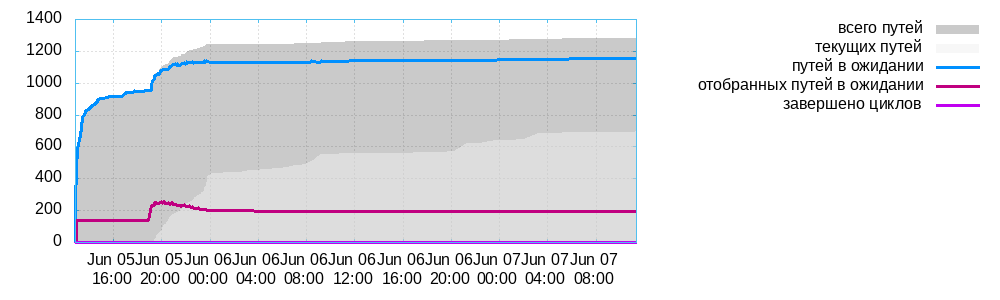
\includegraphics[scale=0.3]{../img/high_freq.png}
    }
    \caption{\tiny{Оригинальный \texttt{AFL}}}
\end{figure}
\begin{figure}[H]
    \center{
        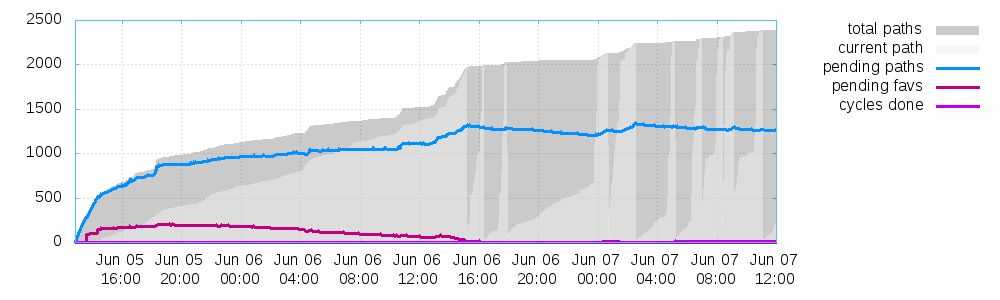
\includegraphics[scale=0.3]{../img/high_freq_moflow.png}
    }
      \caption{\tiny{\texttt{AFL}, использующий \texttt{moflow gentrace}}}
\end{figure}
  \small{Спустя сутки оригинальный AFL практически перестал находить новые пути, а \texttt{AFL}, использующий \texttt{moflow}, открыл еще столько же новых}.
\end{frame}

\begin{frame}{Пример интеграции с фаззером}
\begin{figure}[H]
    \center{
        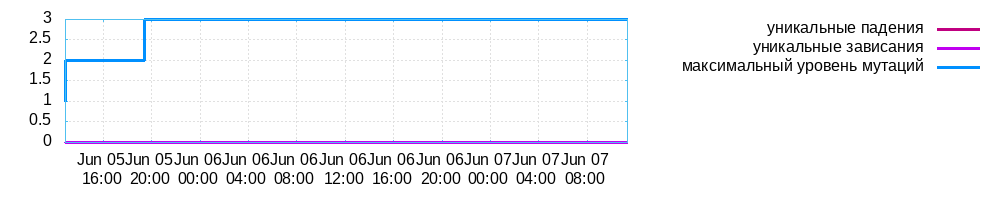
\includegraphics[scale=0.3]{../img/low_freq.png}
    }
    \caption{\tiny{Оригинальный \texttt{AFL}}}
\end{figure}
\begin{figure}[H]
    \center{
        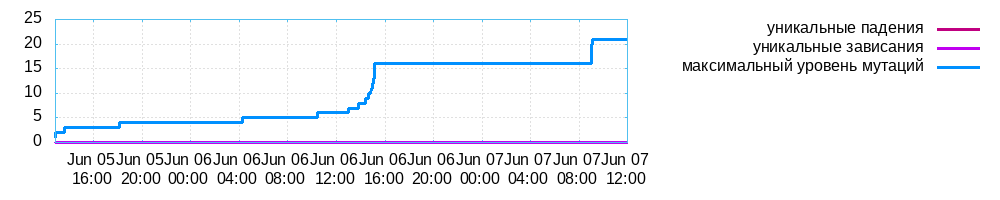
\includegraphics[scale=0.3]{../img/low_freq_moflow.png}
    }
      \caption{\tiny{\texttt{AFL}, использующий \texttt{moflow gentrace}}}
\end{figure}
  \small{Максимальный уровень мутации --- это номер наибольшего поколения мутаций оригинальных входных файлов, на которых открылись новые пути. Большее значение этого параметра в версии с \texttt{moflow gentrace} говорит об улучшении эффективности мутаций}.
\end{frame}

\begin{frame}{Заключение}

\begin{itemize}
\item Выявлены два подхода на основе динамического анализа, позволяющие определять входные данные, влияющие на выполнения условных переходов.
\item Предложены методы на основе динамического символьного анализа и динамического анализа помеченных данных.
\item Методы программно реализованы на инструментах \textbf{Angr} и \textbf{Moflow gentrace}.
\item Реализованные решение протестированы на тестовом наборе \textbf{LAVA} и приложениях с открытым исходным кодом.
\end{itemize}


\end{frame}

\begin{frame}[standout] \vfill Спасибо за внимание \vfill \end{frame}

%\begin{frame}[standout] \vfill Thanks for attention \vfill \end{frame}
\end{document}
